% to show only one bar in the legend
\pgfplotsset{compat=1.11,
    /pgfplots/ybar legend/.style={
    /pgfplots/legend image code/.code={%
       \draw[##1,/tikz/.cd,yshift=-0.25em]
        (0cm,0cm) rectangle (3pt,0.8em);},
   },
}

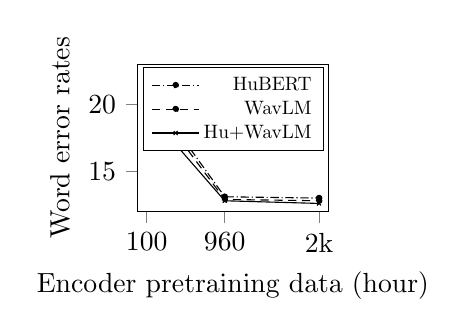
\begin{tikzpicture}
\begin{axis}[
    legend cell align={right},
    legend style={nodes={scale=0.7, transform shape}},
    width=0.33\textwidth,
    tick align=outside,
    tick pos=left,
    xlabel=Encoder pretraining data (hour),
    ylabel= Word error rates,
    xmin=0, xmax=2100,
    ymin=12, ymax=23,
    xtick={100,960, 2000},
    xticklabels={100,960, 2k},   % <---
    ytick={10,4,...,23}
            ]
\addplot[mark=*,black, mark size=1, densely dashdotted] 
plot coordinates {
    (100,21.2)
    (960,13.1)
    (2000,13.0)
};
\addlegendentry{HuBERT}

\addplot[color=black,mark=*, mark size=1, densely dashed]
    plot coordinates {
        (100,20.7)
        (960,12.9)
        (2000,12.8)
    };
\addlegendentry{WavLM}

\addplot[color=black,mark=x, mark size=1]
    plot coordinates {
        (100,19.5)
        (960,12.8)
        (2000,12.6)
    };
\addlegendentry{Hu+WavLM}
\end{axis}
%\caption{WER on test-other}
%\label{fig:werr_pretraining}
\end{tikzpicture}
% ---------------------------------------------------------------------------------------
\begin{tikzpicture}
\definecolor{darkgray176}{RGB}{176,176,176}
\begin{axis}[
legend cell align={left},
legend style={
    nodes={scale=0.7, transform shape},
  fill opacity=1.0,
  draw opacity=1.0,
  text opacity=1,
  at={(0.01,0.99)},
  anchor=north west,
  draw=none
},
width=0.33\textwidth,
tick align=outside,
tick pos=left,
x grid style={darkgray176},
xlabel={Encoder pre-training data (hour)},
xmin=-0.23, xmax=2.63,
xtick style={color=black},
xtick={0.2,1.2,2.2},
xticklabels={100,960,2k},
y grid style={darkgray176},
ylabel={Averaged WERR (\%)},
ymin=0, ymax=40.46875,
ytick style={color=black},
]
\draw[draw=black,fill=white,postaction={pattern=north east lines}] (axis cs:-0.1,0) rectangle (axis cs:0.1,2.08333333333334);
\draw[draw=black,fill=white,postaction={pattern=north east lines}] (axis cs:0.9,0) rectangle (axis cs:1.1,35.0694444444444);
\draw[draw=black,fill=white,postaction={pattern=north east lines}] (axis cs:1.9,0) rectangle (axis cs:2.1,36.1111111111111);
\addlegendimage{ybar,ybar legend,draw=black,fill=white,postaction={pattern=north east lines}}
\addlegendentry{HuBERT}

\draw[draw=black,fill=white,postaction={pattern=north west lines}] (axis cs:1.1,0) rectangle (axis cs:1.3,36.1111111111111);
\draw[draw=black,fill=white,postaction={pattern=north west lines}] (axis cs:2.1,0) rectangle (axis cs:2.3,37.5);
\draw[draw=black,fill=white,postaction={pattern=north west lines}] (axis cs:0.1,0) rectangle (axis cs:0.3,4.86111111111112);
\addlegendimage{ybar,ybar legend,draw=black,fill=white,postaction={pattern=north west lines}}
\addlegendentry{WavLM}


\draw[draw=black,fill=white,postaction={pattern=crosshatch}] (axis cs:1.3,0) rectangle (axis cs:1.5,37.5);
\draw[draw=black,fill=white,postaction={pattern=crosshatch}] (axis cs:2.3,0) rectangle (axis cs:2.5,38.5416666666667);
\draw[draw=black,fill=white,postaction={pattern=crosshatch}] (axis cs:0.3,0) rectangle (axis cs:0.5,9.375);
\addlegendimage{ybar,ybar legend,draw=black,fill=white,postaction={pattern=crosshatch}}
\addlegendentry{Hu+WavLM}

\end{axis}
%\caption{Relative WERRs}
\label{fig:werr_pretraining}
\end{tikzpicture}
% ---------------------------------------------------------------------------------------
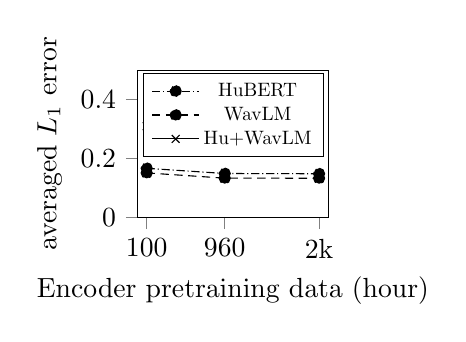
\begin{tikzpicture}
\begin{axis}[
    legend style={nodes={scale=0.7, transform shape}},
    width=0.33\textwidth,
    tick align=outside,
    tick pos=left,
    xlabel=Encoder pretraining data (hour),
    ylabel=averaged $L_1$ error,
    xmin=0, xmax=2100,
    ymin=0, ymax=0.5,
    xtick={100,960, 2000},
    xticklabels={100,960, 2k},   % <---
    ytick={0.1,0.05,...,0.4}
            ]
\addplot[mark=*,black, densely dashdotted] 
plot coordinates {
    (100,0.1667)
    (960,0.1490)
    (2000,0.1482)
};
\addlegendentry{HuBERT}

\addplot[color=black,mark=*, densely dashed]
    plot coordinates {
        (100,0.1511)
    (960,0.1332)
    (2000,0.13302)
    };
\addlegendentry{WavLM}

\addplot[color=black,mark=x]
    plot coordinates {
        (100,0.3095)
    (960,0.2988)
    (2000,0.2972)
    };
\addlegendentry{Hu+WavLM}
\end{axis}
%\caption{$L_1$ error}
\label{fig:l1_err_pretraining}
\end{tikzpicture}
